\documentclass[12pt, a4paper, notitlepage, oneside]{article}
\usepackage[english]{babel}
\usepackage[utf8]{inputenc} 
\usepackage{graphicx}
\usepackage{hyperref}
\usepackage{enumerate}
\usepackage{setspace}

\makeatletter

\newcommand{\linia}{\rule{\linewidth}{0.4mm}}

\renewcommand{\maketitle}{
\begin{titlepage}

    \vspace*{1cm}

    \begin{center}\small

    Warsaw University of Technology\\
    The Faculty of Electronics and Information Technology\\

    \end{center}

    \vspace{3cm}

     \begin{center}

    Data Mining (EDAMI)\\ Project Documentation

    \end{center}

    \noindent\linia

    \begin{center}

      \LARGE \textsc{\@title}

         \end{center}

     \noindent\linia

    \vspace{0.5cm}

    \begin{flushright}

    \begin{minipage}{5cm}

    \textit{\small Authors:}\\

    \normalsize \textsc{\@author} \par

    \end{minipage}

    \vspace{4cm} 
 
     \end{flushright}

    \vspace*{\stretch{6}}

    \begin{center}

    \@date

    \end{center}

  \end{titlepage}
}

\makeatother

\title{Clustering based on density}

\author{Adam Stelmaszczyk\\ Anonymous Coauthor}

\begin{document}

\maketitle
\tableofcontents

\newpage

\section{Project task}
Implementation and experimental evaluation of DBSCAN~\cite{dbscan} and DENCLUE~\cite{denclue} clustering algorithms. 

\section{Data set}

For the experiments a data set with geometrical properties of wheat kernels was chosen,
from the \textit{UCI Irvine Machine Learning Repository}~\cite{dataset}.
Kernels belong to 3 different varieties of wheat: Kama, Rosa and Canadian.
Data set consists of 210 elements, 70 per variety. 

\subsection{Data set attributes information}

Each element consists of 7 real-valued attributes, which are geometric parameters of wheat kernels, 
that were measured using the X-rays: 

\begin{enumerate}
	\item area $A$, 
	\item perimeter $P$, 
	\item compactness $C = \frac{4 \pi A}{P^2}$, 
	\item length of kernel, 
	\item width of kernel, 
	\item asymmetry coefficient 
	\item length of kernel groove. 
\end{enumerate}

\section{Descriptions of used algorithms}
 
Two popular clustering algorithms were used, DBSCAN ~\cite{dbscan} and DENCLUE ~\cite{denclue}. 
In this section brief descriptions of both methods are presented.

\subsection{DBSCAN algorithm}

DBSCAN algorithm is relatively simple algorithm controlled with 2 parameters, namely EPS and MIN\_PTS. \cite{dbscan}
Basically, we are iterating over a set of unvisited points. If we found a core point (a point which has
at least MIN\_PTS in its Eps-neighbourhood), we are starting a new cluster. Looking at the neighbours 
of found core point we are trying to expand this new cluster as much as possible (in respect to the Eps-neighbourhood).

\subsection{DENCLUE algorithm}

DENCLUE algorithm is based on the idea that the influence of each data point can be modeled using a mathematical function (influence function). The overall density of the data space can be calculated as the sum of the influence function of all data points. Clusters can be determined mathematically by identifying density-attractors, which are the local maxima of the overall density function. The DENCLUE algorithm works in two steps:

\begin{enumerate}
	\item Preclustering step, in which a map of the relevant portion of the data space is constructed. The map is used to speed up the calculation of the density function which requires to efficiently access neighboring portions of the data space. 
	
	\item Actual clustering step, in which the algorithm identifies the density-attractors and the corresponding density-attracted points.
\end{enumerate}

\section{Implementation details}

As implementation language for the project Java was chosen.
Data set is read from a \texttt{seeds\_dataset.txt} text file and passed to a standard input of our bechmarking program.
In the benchmark, set of objects that represent points is created. 
DBSCAN and DENCLUE algorithms are using that set.
Other arguments that algorithms need are hard-coded. Whole program consists of five packages:

\begin{itemize}
	\item \texttt{algorithms} In this package abstract class ClusteringAlgorithm and inherited from it classes DBSCAN and DENCLUE are located. 

	\begin{figure}[!ht]
 	\centering
	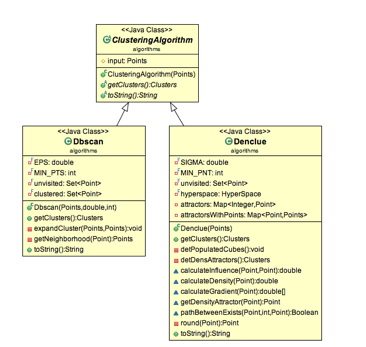
\includegraphics[width=0.8\textwidth]{images/algorithms_package.png}
 	\caption[]
	{Class diagram for algorithms package}
\label{algorithms}
	\end{figure}

	\item \texttt{structures} Here are located basic structure classes like Cluster, Point and Points. Diagram class is shown on the picture~\ref{structures}.

	\begin{figure}[!ht]
 	\centering
	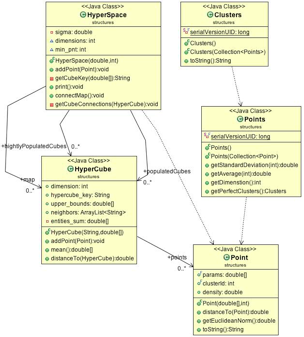
\includegraphics[width=0.7\textwidth]{images/structures_package.png}
 	\caption[]
	{Class diagram for structures package}
\label{structures}
	\end{figure}

	\item \texttt{scorer} This package consists of a Scorer class, which used to calculate clustering quality measure. Diagram class is shown on the picture~\ref{scorer}.

	\begin{figure}[!ht]
 	\centering
	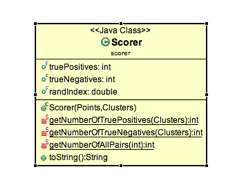
\includegraphics[width=0.4\textwidth]{images/scorer_package.png}
 	\caption[]
	{Class diagram for scorer package}
	\label{scorer}
	\end{figure}

	\item \texttt{visualizer} Used for the clusters visualization. Diagram class is shown on the picture~\ref{visualizer}.

	\begin{figure}[!ht]
 	\centering
	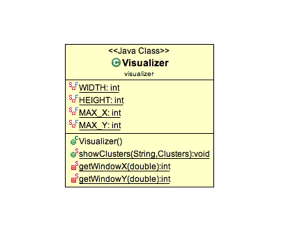
\includegraphics[width=0.35\textwidth]{images/visualizer_package.png}
 	\caption[]
	{Class diagram for visualizer package}
\label{visualizer}
	\end{figure}

	\item \texttt{main} Used for reading the data set from the file and bechmarking algorithms. Diagram class is shown on the picture~\ref{main}.

	\begin{figure}[!ht]
 	\centering
	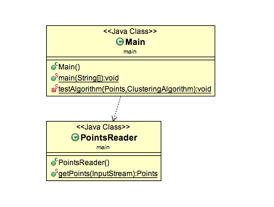
\includegraphics[width=0.45\textwidth]{images/main_package.png}
 	\caption[]
	{Class diagram for main package}
\label{main}
	\end{figure}

\end{itemize}

\section{User guide}

To run benchmark program please follow this 3 steps:

\begin{enumerate}
\item Add execution rights to 2 scripts with a command \texttt{chmod +x build.sh; chmod +x run.sh}.
\item Compile Java source code running \texttt{./build.sh}. \texttt{bin} catalog should appear.
\item Run benchmark program with \texttt{./run.sh}.
\end{enumerate}

\cleardoublepage

\section{Experimentation results and analysis}

As a result of execution DBSCAN and DENCLUE algorithms two sets of clusters are generated. 
This clusters are represented in 2D view as a set of points, drawn as numbers (fig.~\ref{perfect}, ~\ref{dbscan}, ~\ref{denclue}). 
Each number is representing cluster ID. ~\textit{Area} and~\textit{asymmetry coefficient} are on axes,
because this attributes have the greatest standard deviations (fig.~\ref{result}).

\begin{figure}[!ht]
 	\centering
	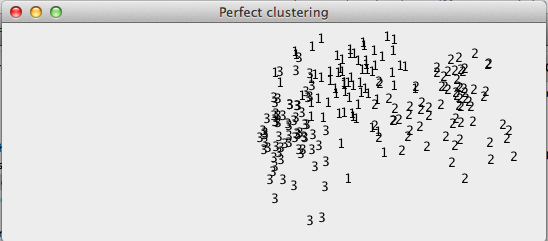
\includegraphics[width=0.6\textwidth]{images/perfect.png}
 	\caption[]
	{Perfect clustering}
	\label{perfect}
	\end{figure}

\begin{figure}[!ht]
 	\centering
	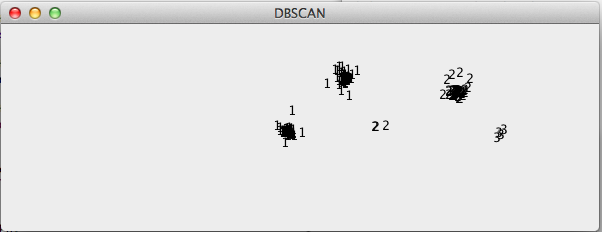
\includegraphics[width=0.6\textwidth]{images/dbscan.png}
 	\caption[]
	{Clustering made by DBSCAN algorithm}
	\label{dbscan}
	\end{figure}

\begin{figure}[!ht]
 	\centering
	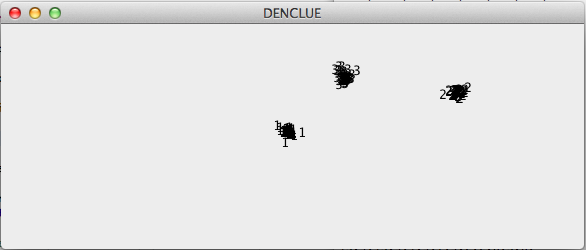
\includegraphics[width=0.6\textwidth]{images/denclue.png}
 	\caption[]
	{Clustering made by DENCLUE algorithm}
		\label{denclue}
	\end{figure}

Also some statistics for the running algorithms are shown, such as number of \textit{true positives}, 
\textit{true negatives} and \textit{Rand index} (picture~\ref{result}).

\begin{figure}[!ht]
 	\centering
	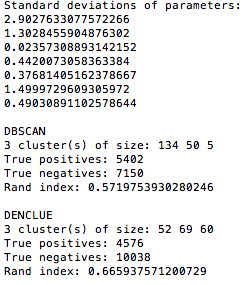
\includegraphics[width=0.35\textwidth]{images/results.png}
 	\caption[]
	{The output of the program}
		\label{result}
\end{figure}

Parameters for the algorithms were chosen experimentally. The best results were achieved using: 
$$EPS = 0.9, MIN\_PTS = 5$$
for DBSCAN and
$$SIGMA = 0.7, EPS = 2$$
for DENCLUE algorithm. \\

It's difficult to measure memory used by algorithms, because of the Java automatic garbage collection, 
which is implementation-specific, nondeterministatic and out of a programmer's control. 
The attempts to calculate free memory before and after the algorithm execution 
were not successful: sometimes there was no difference in the amount of free memory.
Comparison of algorithms running times is presented on figure~\ref{comparison_time}. \\

\begin{figure}[!ht]
 	\centering
	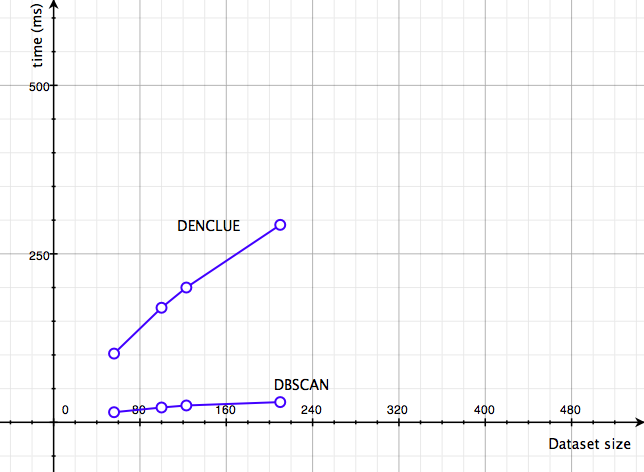
\includegraphics[width=0.7\textwidth]{images/comparison_time.png}
 	\caption[]
	{Comparison of DENCLUE and DBSCAN}
		\label{comparison_time}
\end{figure}

Both algorithms gave different clusterization.
Quality measure (Rand index) was always higher for DENCLUE algorithm.
On the other hand, this algorithm needed more time than DBSCAN to do the same work. 
It should be noticed, that the chosen data set wasn't very big and this difference in time could be different if 
algorithms would try to deal with bigger data sets. 
One could come with a conclustion, that for a bigger data set DENCLUE algorithm will be much more slower 
than DBSCAN, but it's not completely true. 
Time for DBSCAN algorithm in such situation will rise quickly. 
DENCLUE algorithm is dividing data points to cubes, taking for big calculations only highly populated cubes and other elements of the algorithm will make it faster.
On the tested data set DENCLUE algorithm dividing cubes for populated and 
highly populated wasn't a cause of big decrease of considered cubes.
There is also possible optimization for a DBSCAN algorithm, using triangle inequality (TI) property. \cite{mkr}
It could be a vast improvement, because now to calculate a neighbourhood all the points distances are calculated and checked.
With triangle inequality most of the points would be skipped. However, even without this optimization DBSCAN was faster
than DENCLUE, but less accurate, according to our quality measure.

\section{Attribution}

Anonymous Coauthor implemented DENCLUE algorithm, structures essential for it, 
tested memory and time usage and prepared majority of this documenation.
Adam Stelmaszczyk implemented \texttt{scorer}, \texttt{visualizer}, \texttt{main} packages, 
DBSCAN algorithm, structures used in it and wrote part of this documenation.

\newpage

\bibliographystyle{plain}
\bibliography{references}
\end{document}
